j% I USED PDFLATEX TO COMPILE THIS PRESENTATION BECAUSE OF THE
%   GRAPHIC FILE TYPES I HAD.
% IF YOU WOULD LIKE TO COMPILE IT YOURSELF, COMMENT OUT
%   ALL OF THE FIGURES AND MOVIE AND YOU WILL BE ABLE TO
%   COMPILE WITH BOTH PDFLATEX AND LATEX+DVIPS.

\documentclass{beamer}
% \usepackage{pgfpages}
% \setbeameroption{show only notes}
\usetheme{Frankfurt}
\usecolortheme{seahorse}

\usepackage{time}             % date and time
\usepackage{graphicx,epsfig,subcaption}
% \usepackage[T1]{fontenc}      % european characters
\usepackage{amssymb,amsmath}  % use mathematical symbols
\usepackage{textgreek}
% \usepackage{palatino}         % use palatino as the default font
% \usepackage{multimedia}
% \usepackage{mathrsfs}

% CREATES SHADED INSTEAD OF HIDDEN OVERLAYS
\setbeamercovered{transparent}

% package for customizing figures and backgrounds
\usepackage{tikz, chemfig}
\usetikzlibrary{decorations.pathmorphing}
\newcommand{\tn}{\textnormal}
\newcommand{\dd}{d}
\newcommand{\Der}[2]{\frac{\dd #1}{\dd #2}}
\newcommand{\Pder}[2]{\frac{\partial #1}{\partial #2}}
\newcommand{\Int}[4]{\int_{#3}^{#4} #1 \, \dd #2}

\newcommand{\DimReceptorSaturation}{\Int
  {\bondDensity\left(\wallDist,\recAngle,\dTime\right)} {\wallDist}
  {-\infty} {\infty}}
\newcommand{\NDReceptorSaturation}{\Int
  {\ndBondDensity\left(\ndWallDist,\recAngle,\ndTime\right)}{\ndWallDist}
  {-\infty} {\infty}}
\DeclareMathOperator{\Exp}{Exp}
\newcommand{\radius}{R}
\newcommand{\separation}{d}
\newcommand{\stiffness}{k_f}
\newcommand{\boltzmann}{k_B}
\newcommand{\temp}{T}
\newcommand{\onConst}{k_\text{on}}
\newcommand{\offConst}{k_\text{off}}
\newcommand{\refForce}{f_0}
\newcommand{\receptorDensity}{N_T}
\newcommand{\receptorNumber}{N_R}
\newcommand{\appliedRot}{\Omega_f}
\newcommand{\appliedVel}{V_f}
\newcommand{\velFriction}{\xi_V}
\newcommand{\rotFriction}{\xi_\omega}
\newcommand{\compliance}{\Gamma}
\newcommand{\width}{w}
\newcommand{\viscosity}{\mu}

\newcommand{\ndSeparation}{d'}
\newcommand{\ndAppliedRot}{\omega_f}
\newcommand{\ndAppliedVel}{v_f}
\newcommand{\ndOnConst}{\kappa}
\newcommand{\onForceScale}{\eta}
\newcommand{\offForceScale}{\delta}
\newcommand{\ndVelFriction}{\eta_v}
\newcommand{\ndRotFriction}{\eta_\omega}

\newcommand{\ITA}[1]{\textalpha\textsubscript{#1}}
\newcommand{\ITB}[1]{\textbeta\textsubscript{#1}}



\title{Platelet rolling: a simpler approach}
% \subtitle{An Introduction}
\author{Andrew Watson}
\institute{University of Utah} % COMMAND UNIQUE TO BEAMER
\date{\today}

\begin{document}

\begin{frame}
  \titlepage
  \note[item]{Platelet rolling---important first step in the formation
    of blood clots}
  \note[item]{Talk about a simpler approach to modeling rolling that
    Aaron and I have been working on over the summer}
\end{frame}


% %%%%%%%%%%%%%%%%%%%
% \section[Outline]{}
% %%%%%%%%%%%%%%%%%%%
% \begin{frame}
%   \tableofcontents

%   \note{I want to start by talking about the biology behind platelet
%     rolling, and describe some rolling experiments that are being
%     conducted by a biomedical engineering group on campus. Then I'll
%     describe some previous mathematical models of cell rolling, talk
%     about our current model, and finally where we want to go with this
%     model}
% \end{frame}

%%%%%%%%%%%%%%%%%%%
\section{Background}
%%%%%%%%%%%%%%%%%%%

\subsection{Biology of platelet rolling}

\begin{frame}
  \frametitle{Platelet activation}
  \centering
  \includegraphics[width=.8\textwidth]{platelet-overview.png}
  \note[item]{Platelets have to be activated to do all the things
    they do to facilitate blood clot formation}
  \note[item]{Agonists---chemicals that cause platelets to activate}
  \note[item]{Soluble agonists released into the bloodstream}
  \note[item]{Immobilized agonists are bound to the vessel wall or
    to platelets. Because these chemical signals don't diffuse in
    the blood, platelets have to be close enough to a surface to
    bind.}
  \note[item]{}
  \note[item]{Immobilized agonists are exposed on damaged vessels;
    not present on healthy vessels}
\end{frame}

% \begin{frame}
%   \frametitle{Platelet transport to the vessel wall}
%   \begin{itemize}
%     \note[item]{A natural question is how to platelets get transported
%       to the vessel wall?}
%   \item Margination---RBCs push platelets to the edge of the vessel
%   \item High platelet concentration near the wall
%   \end{itemize}

%   \begin{figure}
%     \centering
%     \includegraphics[width=\textwidth]{fl-layer}
%     \caption{Margination transports platelets from the interior of the
%     blood vessel to the vessel wall}
%     \label{fig:marg-plts}
%   \end{figure}
%   \note[item]{In steady state blood flow, the distribution of cells
%     looks like this, with RBCs occupying the center of the vessel, and
%     platelets concentrated near the vessel wall.}
%   \note[item]{If this vessel wall has immobilized agonists exposed,
%     platelets can roll along it.}
% \end{frame}

\begin{frame}
  \frametitle{Activation through rolling}
  \begin{columns}
    \begin{column}{.49\textwidth}
      \begin{itemize}
      \item Fast receptors---transient binding \& rolling
        \note[item]{``Fast receptors''---receptors with fast binding
          and unbinding kinetics; form bonds quickly while the
          platelet is moving past the wall, but are short-lived}
      \item Agonist-receptor bonds trigger activation signals
        \note[item]{When the receptor is bound to an agonist, it
          triggers intracellular activation signals}
        \note[item]{Enough binding events with the agonist causes the
          platelet to activate}
      \item Slow receptors---firm adhesion
        \note[item]{Platelets also have slow receptors. Part of
          platelet activation involves activation of these slow
          receptors, which mediate stable adhesion.} 
      \item Examples: fast receptor---GP1b, slow
        receptor---\ITA{IIb}\ITB{3}, agonist---vWF
      \end{itemize}
      \note[item]{Be sure to distinguish between transient binding
        and firm adhesion}
    \end{column}
    \begin{column}{.49\textwidth}
      \begin{figure}
        \centering
        \includegraphics[width=\textwidth]{transient-binding}
        \caption{An example of a platelet binding to an immobilized
          agonist}
        \label{fig:transient-binding}
      \end{figure}
      \note[item]{The figure on right shows an example of a
        platelet transiently binding to an immobilized agonist
        vWF. The unbound platelet has fast receptors (GP1b) and
        inactive slow receptors (\ITA{IIb}\ITB{3}). The GP1b can bind
        to the vWF, and trigger platelet activation, causing the slow
        \ITA{IIb}\ITB{3} receptors to activate.} 
    \end{column}
  \end{columns}
\end{frame}

% \begin{frame}
%   \frametitle{Rolling dynamics}
%   \note[item]{So what influences the physical process of rolling?}
%   \begin{itemize}
%   \item When a bond forms between a platelet and agonist, a stretching
%     force is applied along the bond as the platelet is pushed by the
%     blood flow
%   \item Bonds can withstand some pulling force, and so slow down the
%     platelet
%     \note[item]{Bonds slow down the platelet as they get stretched}
%   \item Dynamics of a rolling platelet are influenced by:
%     \note[item]{There are several things that drive or influence the
%       rolling behavior of the platelet}
%     \begin{itemize}
%     \item Drag forces imposed by the fluid
%       \note[item]{Drag forces drive the platelet downstream}
%     \item Forces exerted by platelet-agonist bonds
%     \item Nonspecific colloidal forces (gravity, electrostatic, etc.)
%       \note[item]{Most significant is electostatic, cell membranes
%         tend to be negatively charged and so platelet and vessel wall
%         repel each other. Is this true in Dr. Hlady's experiments?}
%     \item Collisions with other cells
%     \item Activation state of the platelet (are any slow receptors
%       active?)
%       \note[item]{In particular, whether there aare any slow receptors
%         active.}
%       \note[item]{That is, the behavior of a rolling platelet can
%         change over time}
%     \end{itemize}
%   \item In summary, activation by rolling is a complicated process
%     involving biophysics and chemistry
%   \end{itemize}
% \end{frame}

% \begin{frame}
%   \frametitle{Rolling dynamics}
%   \begin{figure}
%     \centering
%     \includegraphics[width=\textwidth]{rolling-forces.png}
%     \caption{Forces involved in cell rolling}
%     \label{fig:rolling-forces}
%   \end{figure}
%   \note[item]{What influences the physical process of rolling?}
%   \note[item]{Bonds form with wall, get stretched as the platelet
%     moves downstream, exert force}
%   \note[item]{Drag force from fluid}
%   \note[item]{Colloidal forces act on the platelet. Most significant
%     is electrostatic}
%   \note[item]{Collisions with other cells can occur}
%   \note[item]{Platelet can influence its rolling by activating slow
%     receptors} 
%   \note[item]{Activation by rolling is complicated process: biophysics
%     and chemistry}
% \end{frame}

% \begin{frame}
%   \frametitle{Summary of rolling biology}
%   \begin{itemize}
%     % \item Platelets get pushed towards vessel walls
%   \item Platelets are activated by agonists
%     \vfill
%   \item Immobilized agonists exposed on injured vessels
%     \vfill
%   \item Platelets transiently contact agonist on the wall---platelet
%     activation and begin clotting process
%   \end{itemize}
%   \note[item]{This is also an important consideration in the
%     engineering of medical devices that get placed into the
%     bloodstream.}
% \end{frame}

% \subsection{Rolling experiments}

% \begin{frame}
%   \frametitle{Hemocompatibility}
%   \begin{itemize}
%   \item This rolling behavior is relevant in the design of
%     biomaterials for blood-contacting devices
%   \item Implanted devices are a common treatment for cardiovascular
%     diseases, must be designed to not elicit an immune or clotting
%     response 
%   \item Current designs still have negative side-effects: patients
%     must be placed on systemic anti-coagulants

%     \note[item]{``Primed'' meaning that it takes less stimulus for a
%       platelet to reach full activation (whatever that means) than a
%       completely inactive platelet}
%   \end{itemize}
% \end{frame}

% \begin{frame}
%   \frametitle{Hemocompatibility}
%   \centering
%   \begin{tikzpicture}
  \pgftext{\includegraphics[width=.75\textwidth]{blood-vessel}}
  \draw[very thick, ->] (-3, 2.6) -- node[fill=white] {flow direction} +(5,.35);
  \draw[thick, ->] (-3.5, -3.5) node[below] {Native vessel} -- ++(0, 1);
  \draw[thick, ->] (1, -3.3) node [below] {Artificial vessel} -- ++(0, 1);
  \draw[thick, ->] (-1, -4) node[below] {Anastomoses} .. controls (-1, -2) .. +(-1.5, 3);
  \draw[thick, ->] (-.8, -4) .. controls (-.8, -2) and (0, -1) .. +(2.5, 3.5);
\end{tikzpicture}

%   \note[item]{Implanted devices are a common treatment for
%     cardiovascular diseases, must be designed to not elicit an immune
%     or clotting response}
%   \note[item]{Current designs still have negative side-effects:
%     patients must be placed on systemic anti-coagulants}
%   \note[item]{Inherent nonlocality in implanted
%     devices}
%   \note[item]{Here is an example of a vascular graft.}
%   \note[item]{ECs unhappy in anastomotic regions}
%   \note[item]{There can be exposed agonists in these regions,
%     the vessel might narrow.}
%   \note[item]{Immobilized agonists can also bind to the biomaterial
%     itself.} 
%   \begin{itemize}
%   \item Implanted devices---common treatment for cardiovascular
%     diseases
%   \item Current designs have negative side effects---require systemic
%     anticoagulants 
%   \end{itemize}
% \end{frame}

\begin{frame}
  \frametitle{Rolling experiments}
  \begin{figure}
    \centering
    \includegraphics[width=.75\textwidth]{expt-sideview}
    \caption{Side view of the priming microfluidic
      chambers. Eichinger, Ph.D. dissertation, 2016.}
    \label{fig:flow-chamber}
  \end{figure}

  \begin{itemize}
  % \item A research group in biomedical engineering led by Dr. Hlady is
  %   studying the nonlocal effects of platelet interaction with
  %   immobilized agonists
    \note[item]{Activation of platelets through rolling is an
      important concern in biomedical engineering as well}
    \note[item]{Artificial devices implanted in the blood must be
      engineered to not trigger immune or clotting responses}
  % \item Nonlocal effects---experiments from
  %   Proteins-Polymers-Interfaces group led by Dr. Hlady
  % \item Basic idea: platelets can transiently bind to agonists without
  %   firmly adhering, and be primed for full activation downstream
  \item Question: how does priming (i.e. previous exposure to agonist)
    affect rolling behavior?
  \item Setup:
    $\tn{Control} = \tn{Unprimed (inert material in priming region)}$
    vs $\tn{Experimental} = \tn{Primed (agonist in priming region)}$
  \item Data extracted: platelet velocities, step sizes, pause
    times 
  \end{itemize}
  \note[item]{This general setup underpins several different
    experiments they are carrying out. Essentially there are two
    regions printed with agonist, and platelets get primed in the
    upstream region, and then are more likely to adhere to the surface
    downstream in the capture region.}
  \note[item]{They have a set of experiments looking at how priming
    state affects rolling behavior.}
  \note[item]{Extract the following data...}
\end{frame}

% \begin{frame}
%   \frametitle{Idealized platelet trajectory}
%   \note[item]{Here is an idealized platelet trajectory to illustrate
%     step sizes and pause times}
%   \begin{figure}
%     \centering \includegraphics[width=.75\textwidth]{steps-pauses}
%     \caption{Examples of step size, pause time, and average velocity.}
%     \label{fig:plt-trajectory}
%   \end{figure}
% \end{frame}

\begin{frame}
  \frametitle{Example platelet trajectories}
  \note[item]{Here is an idealized platelet trajectory to illustrate
    step sizes and pause times}
  \begin{figure}
    \centering \includegraphics[width=.75\textwidth]{plt-trajectories}
    \caption{Examples of platelet trajectories from a single
      experiment. Resolution: ($\Delta t = 80 \tn{ms}$, $\Delta x
      \approx 150\tn{nm} \tn{, maybe?}$)}
    \label{fig:plt-trajectory}
  \end{figure}
  \note[item]{Our goal: simulate platelet trajectories, get some mechanistic
    insight into the rolling process}
\end{frame}

% \begin{frame}
%   \frametitle{Results of priming}
%   \begin{figure}
%     \centering
%     \includegraphics[width=.75\textwidth]{expt-sideview}
%     \caption{Side view of the priming microfluidic
%       chambers. Eichinger, Ph.D. dissertation, 2016.}
%   \end{figure}
%   \begin{itemize}
%   \item Result: Primed platelets have slower average velocity and
%     smaller step sizes (unpublished data)
%   \item Modeling motivation: directly observing bonds between the
%     platelet and wall is not feasible
%     \note[item]{Rolling behavior is observable, the number of bonds is
%       not. But the number of bonds affects how much a platelet gets
%       primed, and the number of slow receptors active on the surface
%       is the result of the primed state}
%   \item Modeling connects observable data to bond numbers, bond
%     lifetimes, primed state
%   \end{itemize}
% \end{frame}

% \begin{frame}
%   \frametitle{Rolling experiments}
%   \begin{center}
%     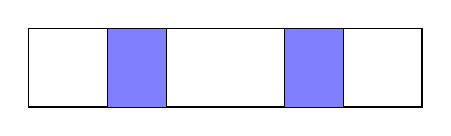
\begin{tikzpicture}[scale=.5]
  \draw[semithick] (-5, -1) rectangle (5, 1);
  \filldraw[fill=blue!50] (-3, -1) rectangle (-1.5, 1);
  \filldraw[fill=blue!50] (1.5, -1) rectangle (3, 1);
\end{tikzpicture}
    
%   \end{center}

%   \begin{itemize}
%   \item Video camera placed in the downstream region to capture
%     rolling behavior of platelets
%   \item Data extracted: instantaneous velocities of rolling platelets,
%     pause times (the length of time a platelet is stationary), and
%     step sizes (the distance traveled in between two pauses)
%   \item They found that priming reduces the average rolling velocity
%     of platelets, but also unprimed platelets seemed to separate into
%     2 subpopulations: one group was moving slowly, and one group was
%     moving more quickly (the frequency plot of velocities is bimodal)
%   \end{itemize}
%   \note{Define jumps and pauses here?}
% \end{frame}

% \subsection{Previous mathematical models}

% \begin{frame}
%   \frametitle{Previous rolling models}
%   \centering
%   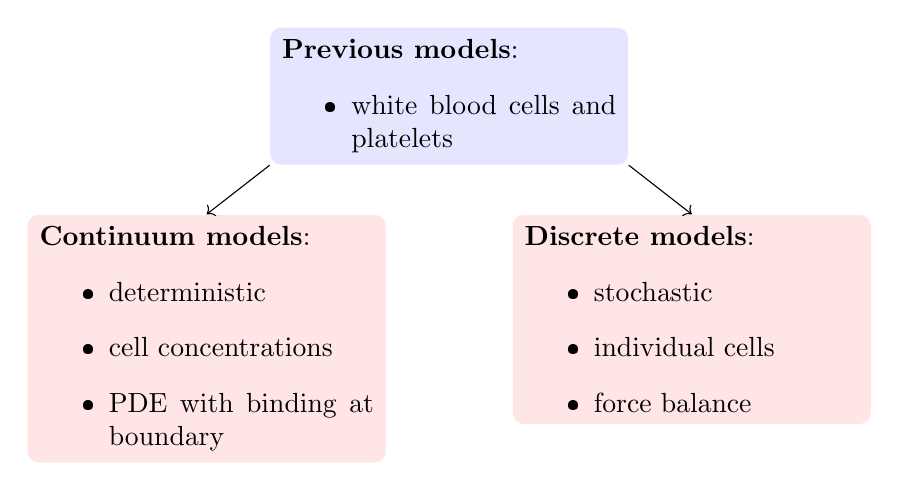
\begin{tikzpicture}
  \node (root) at (0, 0)
  [rounded corners, fill=blue!10, inner sep=1ex]
  {
    \begin{minipage}{.35\linewidth}
      \textbf{Previous models}: 
      \begin{itemize}
      \item white blood cells and platelets
      \end{itemize}
    \end{minipage}
  };
  
  \node (left child) at (-.8, -1.5)
  [below left, rounded corners, fill=red!10, inner sep=1ex]
  {
    \begin{minipage}{.35\linewidth}
      \textbf{Continuum models}: 
      \begin{itemize}
      \item deterministic
      \item cell concentrations
      \item PDE with binding at boundary
      \end{itemize}
    \end{minipage}
  };
  
  \node (right child) at (.8, -1.5)
  [below right, rounded corners, fill=red!10, inner sep=1ex]
  {
    \begin{minipage}{.35\linewidth}
      \textbf{Discrete models}: 
      \begin{itemize}
      \item stochastic
      \item individual cells 
      \item force balance
      \end{itemize}
    \end{minipage}
  };

  \draw[->] (root.south west) -- (left child.north);
  \draw[->] (root.south east) -- (right child.north);
\end{tikzpicture}

%   \begin{itemize}
%   \item Goal: use stochastic modeling to reproduce rolling data
%   \end{itemize}
%   \note[item]{Rolling models are diverse, models with a wide range of
%     assumptions, usually model white blood cells or platelets}
%   \note[item]{One way to separate them is in whether they model cells
%     as a continuum or as discrete entities}
%   \note[item]{Only a stochastic model of individual cells can be used
%     to reproduce the rolling data being collected. There is no concept
%     of steps or pauses in a deterministic model.}
%   \note[item]{To illustrate models of the discrete-cell stochastic
%     type, describe an early cell rolling model called Adhesive
%     Dynamics}
% \end{frame}

% \begin{frame}
%   \frametitle{Previous rolling models}
%   \begin{itemize}
%   \item Cell rolling and adhesion models are diverse, have a wide
%     range of assumptions, and usually model either white blood cells
%     or platelets
%     \note[item]{This makes it hard to characterize rolling models as a
%       whole. But one important distinction to make between models is
%       whether they treat cells as individuals or as a population.}
%   \item On the simpler end: populations of cells modeled as a
%     continuum. These tend to model cell concentrations in the blood as
%     a PDE, with a boundary on the wall to capture binding and
%     unbinding
%   \item On the more complicated end: cells modeled individually, often
%     bond formation is stochastic, calculate fluid forces and bond
%     forces to determine rolling velocity
%     \note[item]{We want a model that simulates the velocity of
%       individual cells to match with experimental data. In a
%       continuous deterministic model, there are no steps or pauses, so
%       our rolling model should model the behavior of an individual
%       platelet with random transient contacts with the surface}
%   \end{itemize}
% \end{frame}

% \begin{frame}
%   \frametitle{Adhesive dynamics (AD) model (Hammer \& Apte, 1992)}
%   \note[item]{AD models are a common family of models with
%     modifications for many different situations. Original model was
%     published by Hammer and Apte in 1992.}
%   \begin{columns}
%     \begin{column}{.49\textwidth}
%       \begin{itemize}
%       \item 3D stochastic rolling model of individual white blood cells
%       \item Model components:
%         \begin{enumerate}
%         \item Cell body is a rigid sphere with receptors
%         \item Random length dependent binding \& unbinding with wall
%         \item Steady Stokes flow
%         \item 3 types of forces: drag force, bond force, and colloidal
%           forces
%         \end{enumerate}
%         \note[item]{Randomness comes from bond formation and breaking,
%           cell motion is deterministic b/c it's determined by Stokes
%           flow}
%         \note[item]{Bonds are identified by their two endpoints}
%         \note[item]{Time is advanced in the model by drawing from
%           Poisson distributed random variables to determine which
%           reactions occur, and then calculating the velocity of the
%           cell from Stokes flow and updating its position}
%       \end{itemize}
%     \end{column}
%     \begin{column}{.49\textwidth}
%       \begin{figure}
%         \centering
%         \includegraphics[width=\textwidth]{hammer92scr.jpg}
%         \caption{Diagram of a cell in the AD model from Hammer \&
%           Apte, 1992.}
%         \label{fig:hammer-scr}
%       \end{figure}
%     \end{column}
%   \end{columns}
% \end{frame}

% \begin{frame}
%   \frametitle{Proposed model}
%   \begin{itemize}
%   \item The AD model is able to reproduce observed rolling behavior of
%     white blood cells
%     \vfill
%   \item Limitations: detailed and expensive to run
%     \vfill
%   \item Proposed model: reduction to 2D, simplify forces involved
%     \note[item]{With the proposed model, we want to reduce the AD
%       model to 2D ...}
%     \vfill
%   \item Goal: develop a reduced model suited for experimental
%     comparison and validation
%   \end{itemize}
% \end{frame}

%%%%%%%%%%%%%%%%%%%
\section{Models: Old and New}
%%%%%%%%%%%%%%%%%%%

% \subsection{Model assumptions}

% \begin{frame}
%   \frametitle{Modeling assumptions}
%   \begin{enumerate}
%   \item 2D steady Stokes flow
%     \note[item]{Mention Stokes flow implies that there is a linear
%       relationship between the platelet translation and angular
%       velocity and the drag force and torque}
%     \vfill
%   \item Platelet is a rigid sphere with uniformly distributed
%     receptors
%     \vfill
%   \item The reactive region is approximated as a cylinder
%     \note[item]{The reactive region is the portion of the platelet
%       surface close enough to the wall for bonds to form.}
%     \note[item]{Approximating the reactive region as a cylinder means
%       the model can be reduced to 2D}
%     \vfill
%   \item Platelet only moves parallel to the wall
%     \vfill
%   \item Separation distance from the wall is constant
%     \vfill
%   \item Forces and torques: drag force (fluid) and bond force (linear spring)
%     balance
%     \note[item]{Force balance is also a consequence of steady stokes
%       flow} 
%   \end{enumerate}
% \end{frame}

\begin{frame}
  \frametitle{Detailed Rolling Model}
  \note[item]{Those assumptions give us a picture that looks like
    this}
  \note[item]{Platelet has radius $\radius$}
  \note[item]{Platelet moves with translational velocity $\velocity$
    and angular velocity $\rotation$}
  \note[item]{It is sitting in a shear flow with shear rate $\shear$}
  \note[item]{Separated from the wall by distance $\separation$}
  \note[item]{Bonds form between the platelet and wall, and are
    identified by their two endpoints}
  \note[item]{The platelet endpoint is identified by the coordinate
    $\recAngle$, angle from the downward vertical}
  \note[item]{Wall endpoint is identified by $\wallDist$, the distance
    along the wall from the center of the platelet.}
  \note[item]{First question, how to determine $\velocity$ and $\rotation$?}
  \begin{figure}
    \centering
    \begin{tikzpicture}[scale=2]
  \newcommand{\dist}{0.5}
  \newcommand{\Length}{2.5}
  \newcommand{\slope}{0.5}
  \newcommand{\buff}{0.1}

  % Define a coordinate for the center of the platelet, and draw a
  % node there
  \coordinate (pltcenter) at (0, 1 + \dist);
  \node [circle, inner sep=1.5pt, fill=black] at (pltcenter) {};

  % Draws the wall and the platelet
  \draw (-\Length, 0) -- (\Length, 0);
  \draw (pltcenter) circle [radius = 1];
  \draw[<->] (0, .05) -- node[right] {$\separation$} (0, \dist-.05);
  \draw[<->] (-.15, .05) -- node[left] {$\height$} (-.15,
  .95+\dist);
  \draw[dashed] (0, 1+\dist) -- (-.3, 1+\dist);

  % Draws the lines showing the applied velocities
  \draw[->] (pltcenter) ++(1+\buff, 0) -- node[above] {$\velocity$}
  (\Length-\buff, 1+\dist);

  \draw[->] (0, 1+\dist) ++(135:1+\buff) arc [start angle=135, end
  angle=45, radius=1+\buff] node[midway, above] {$\rotation$};

  % Draws the arrows showing the shear flow
  \foreach \y in {0.5, 1, 1.5, 2, 2.5}
     \draw[->] (-\Length, \y) -- (-\Length + \slope*\y, \y);
  
  \draw[gray, very thin] (-\Length, 0) -- node[near start, right,
  black] {$\tn{Shear rate} = \shear$} (-\Length + \slope*\Length,
  \Length);

  % Draws a bond between the platelet and wall
  \draw[decorate, decoration=zigzag] (pltcenter) ++(315:1)
  node[circle, inner sep=1.5pt, fill=black] {} -- (1.25,0) node
  [circle, inner sep=1.5pt, fill=black] {};

  % Labels the x and theta coordinates
  \draw[{Bar[]}->] (0, -\buff) -- node[fill=white] {$\wallDist$}
  (1.25, -\buff);

  \draw (pltcenter) -- +(0, -1);
  \draw (pltcenter) -- node[above right] {$R$} +(315:1);
  \draw[->] (pltcenter) ++(0, -3*\buff) arc [start angle=270, end
  angle=315, radius=3*\buff] node[midway, below] {$\recAngle$};
\end{tikzpicture}

    \caption{Geometry of the rolling model}
    \label{fig:model-geom}
  \end{figure}
\end{frame}

\begin{frame}
  \frametitle{Results from the detailed model}
  \begin{itemize}
  \item Exhibits stepping and pausing behavior
  \item Sensitive to priming
  \item Weaknesses
    \begin{itemize}
    \item Model uses unknown and hard to estimate parameters
    \item Too expensive to fit parameters, and too complex for the
      data available
    \end{itemize}
  \end{itemize}
\end{frame}

\begin{frame}
  \frametitle{What is the simplest possible model?}
  \begin{figure}
    \centering
    \includegraphics[width=.75\textwidth]{jump-velocity-sketch}
    \caption{A simple stochastic binding model}
    \label{fig:jump-velocity-sketch}
  \end{figure}

  \begin{figure}
    \centering
    \schemestart
    U \arrow{<=>[$\beta$][$\alpha$]} V
    \schemestop\par
    \caption{Two-state reaction diagram for the binding model}
    \label{fig:two-state-scheme}
  \end{figure}
\end{frame}

\begin{frame}
  \frametitle{A brief description}
  \begin{center}
    \schemestart
    U \arrow{<=>[$\beta$][$\alpha$]} V
    \schemestop\par    
  \end{center}
  \begin{itemize}
  \item Stochastic switching between states U and V with constant
    rates $\alpha$ and $\beta$.
  \item When the platelet is in state U, it translates with velocity
    $=1$, while platelets in the V state remain stationary.
  \item Defines a stochastic process called a jump-velocity process
  \item Easy to define quantities analogous to the experimental data:
    average velocity (of a single trajectory), step sizes, pause times
  \end{itemize}
\end{frame}

\begin{frame}
  \frametitle{Average velocity}
  \begin{itemize}
  \item To get average velocity, we need the Fokker-Planck equation of
    the stochastic process
  \item The Fokker-Planck equation for the two-state model:
    \begin{align}
      \Pder{p_U}{t} &= -\Pder{p_U}{x} - \beta p_U + \alpha p_V \\
      \Pder{p_V}{t} &= \beta p_U - \alpha p_V
    \end{align}
  \item $p_i(x, t)$ is the probability that at time $t$, a platelet is
    in position $x$ and state $i$.
  \item Initial condition: $p_U(x, 0) = \delta(x)$, $p_V(x, 0) = 0$.
  \item Distribution of crossing times = $p_U(1, t)$, then
    distribution of average velocities can be derived
  \end{itemize}
\end{frame}

\begin{frame}
  \begin{figure}
    \centering
    \includegraphics[width=.75\textwidth]{jump-velocity-figure6.pdf}
    \caption{Sample fit of average velocity to simulated data}
    \label{fig:avg-vel-fit}
  \end{figure}
\end{frame}

\begin{frame}
  \frametitle{Four state model}
  \begin{itemize}
  \item Motivation: rolling is mediated by two types of receptors,
    fast receptors and slow receptors
  \item The two state model may be a good model of unprimed platelets,
    because the slow receptors aren't activated
  \item The four state model may be a better choice for primed
    platelets
  \item The Fokker-Planck equation is similar to the two-state model,
    there are just 2 extra equations and a few more reaction terms
  \end{itemize}
  \begin{center}
    \schemestart
    U \arrow{<=>[$\beta$][$\alpha$]}
    V \arrow{<=>[*{0}$\delta$][*{0}$\gamma$]}[270]
    VF \arrow{<=>[$\beta$][$\alpha$]}[180]
    F \arrow{<=>[*{0}$\gamma$][*{0}$\delta$]}[90]
    \schemestop\par
  \end{center}
\end{frame}

\begin{frame}
  \frametitle{Step size}
  \begin{itemize}
  \item In both models, we expect the step sizes to be exponentially
    distributed.
  \item Define $\mathcal{S}$ to be the step size random variable, then
    \begin{itemize}
    \item $\mathcal{S} \sim \Exp(\alpha)$ in the two-state model, and
    \item $\mathcal{S} \sim \Exp(\alpha + \gamma)$ in the four-state model.
    \end{itemize}
  \item Fit experimental step size data to an exponential distribution
  \end{itemize}
\end{frame}

\begin{frame}
  \begin{figure}
    \centering
    \begin{subfigure}{0.48\textwidth}
      \includegraphics[width=\textwidth]{jump-velocity-figure31.pdf}
    \end{subfigure}
    \hfill
    \begin{subfigure}{0.48\textwidth}
      \includegraphics[width=\textwidth]{jump-velocity-figure32.pdf}
    \end{subfigure}
    \caption{Maximum likelihood fit of an exponential model to step
      size data of primed platelets ($N=76$). The Anderson-Darling
      goodness-of-fit test rejects the hypothesis that the steps are
      exponentially distributed ($p < 0.01$). The plots for the other
      available data are similar (but have fewer data points).}
    \label{fig:step-fit}
  \end{figure}
\end{frame}

\begin{frame}
  \begin{figure}
    \centering
    \includegraphics[width=.75\textwidth]{jump-velocity-figure33.pdf}
    \caption{Log plot of $1 - \tn{CDF}$}
    \label{fig:log-cdf}
  \end{figure}
\end{frame}

\begin{frame}
  \frametitle{Where to next?}
  \begin{itemize}
  \item A simple one-step model of binding doesn't seem to be an
    accurate model
  \item Based on the log plot, step sizes distributed as a sum of
    exponentials may be plausible, but how do we get there?
    \begin{enumerate}
    \item If there is a mixture of primed and unprimed platelets, then
      the step sizes will be distributed as a sum of exponentials. But
      why aren't the step sizes in the unprimed experiment
      exponential?
    \item In the detailed rolling model, multiple bonds can form
      between the platelet and surface, and so small steps can occur
      without having the platelet fully detach. How are steps
      distributed in the detailed model?
    \end{enumerate}
  \end{itemize}
\end{frame}

% \begin{frame}
%   \frametitle{Determining translational ($\velocity$) and angular
%     ($\rotation$) velocities}
%   \begin{itemize}
%   \item Assume $\separation \gg \radius$
%     \note[item]{The assumption $\separation \gg \radius$ is an
%       assumption of convenience, but in the model $\separation$ is
%       taken small relative to $\radius$.}
%     \note[item]{From this assumption, the force and torque balance
%       equations are}
%   \item Force and torque balance equations:
%     \begin{align*}
%       0 &= \velFriction (\appliedVel - \velocity) + \horzTotalForce \\
%       0 &= \rotFriction (\appliedRot - \rotation) + \totalTorque
%     \end{align*}
%     \note[item]{The first term in each of these equations gives the
%       drag force from the fluid.}
%     \note[item]{The two $\xi$s are friction coefficients, and they are
%       given by Stokes drag law}
%   \item Stokes' drag law implies
%     $\velFriction = 6 \pi \viscosity \radius$ and
%     $\rotFriction = 8 \pi \viscosity \radius^2$
%     \note[item]{$\appliedVel$ and $\appliedRot$ are the translational
%       and rotation velocities of a platelet flowing freely, not
%       attached to the wall.}
%   \item With a shear rate $\shear$,
%     $\appliedVel = (\radius + \separation)\shear$ and
%     $\appliedRot = \shear/2$  
%   \item $\horzTotalForce$---total bond horizontal force
%   \item $\totalTorque$---total bond torque
%   \end{itemize}
% \end{frame}

% \begin{frame}
%   \frametitle{Binding and unbinding rates}
%   \note[item]{Next, to model binding and unbinding we need rates}
%   \note[item]{Rates should be length-dependent}
%   \begin{itemize}
%   \item Unbinding rate comes from the Bell model (1978):
%     \begin{equation*}
%       \offRate(\length) = \offConst 
%       \exp\left(\frac{\stiffness\length}{\refForce}\right)
%     \end{equation*}
%     \note[item]{Bonds are slip bonds; as their length increases, the
%       breaking rate increases}
%     \vfill
%   \item Binding rate comes from assuming the head of the receptor is
%     diffusing in space:
%     \begin{equation*}
%       \onRate(\length) = \onConst
%       \exp\left(-\frac{\stiffness\length^2}{2 \boltzmann \temp}\right)
%     \end{equation*}
%     \note[item]{On rate assumes the head of the receptor is attached
%       to a spring and is diffusing in space. Hence you end up with
%       this Gaussian form.}
%     \note[item]{As the length $L$ increases, the on-rate decreases and
%       the off-rate increases}
%   \end{itemize}
%   \note[item]{Transition: from these assumptions we derive a
%     stochastic model, and a deterministic model which is a mean-field
%     model of the stochastic one. I'll start by describing the
%     deterministic model.}
% \end{frame}

% \subsection{Deterministic and stochastic models}

% \begin{frame}
%   \frametitle{Deterministic model}
%   \begin{itemize}
%   \item Domain: $\wallDist \in (-\infty, \infty)$,
%     $\recAngle \in [-\pi/2, \pi/2]$
%     \note[item]{Assume that bonds can only form from the lower half of
%       the platelet}
%   \item Bond density ($\bondDensity$) equation:
%     \begin{multline*}
%       \Pder{\bondDensity}{\dTime} =
%       \underbrace{\rotation\Pder{\bondDensity}{\recAngle} +
%         \velocity\Pder{\bondDensity}{\wallDist}}_\tn{Platelet motion}
%       + \underbrace{\onRate(\length) \left(\receptorDensity -
%           \DimReceptorSaturation\right)}_\tn{Bond formation} \\
%       - \underbrace{\offRate(\length) \bondDensity}_\tn{Bond breaking}
%     \end{multline*}
%     \note[item]{First two advection terms come from the motion of the
%       platelet, the next two terms are bond formation and
%       breaking. $\receptorDensity$ is the density of receptors on the
%       surface of the platelet, and the integral term just says that
%       the density of bonds on the platelet surface cannot exceed the
%       density of receptors}
%     \note[item]{V and Omega are unknowns in the model, and are
%       determined by the force balance equations}
%   \item Boundary conditions: $\bondDensity(\wallDist, \recAngle,
%     \dTime) \vert_{\recAngle = \pi/2} = \bondDensity(\wallDist,
%     \recAngle, \dTime) \vert_{\wallDist \rightarrow \infty} = 0$
%   \item Initial condition: $\bondDensity(\wallDist, \recAngle, 0) = 0$
%   \end{itemize}
%   \note[item]{The three unknowns in this set of equations are the bond
%     density $\bondDensity$, the translation velocity $\velocity$, and
%     the rotation rate $\rotation$}
%   \note[item]{Deterministic model can't capture distributions of
%     velocity, there is no concept of pauses and jumps in the
%     deterministic model. Tracking individual bonds allows jumping and
%     pausing to happen.}
% \end{frame}

% \begin{frame}
%   \frametitle{Stochastic model}
%   % Randomness comes from stochastic bond formation and breaking, the
%   % force and torque balance equations remain the same. Clarify: I
%   % call this the stochastic model, it is really piecewise
%   % deterministic 
%   \note[item]{Randomness comes from stochastic bond formation and
%     breaking. In between bond formation or breaking events, the
%     evolution of the model is deterministic}
%   \begin{itemize}
%   \item Bond formation and breaking occurs randomly with rates
%     $\onRate(\length)$ and $\offRate(\length)$
%   \item Discretize platelet surface into $\recAngle$-bins
%   \item Receptors are all located at bin midpoints $\binMidpoint{j}$
%     \note[item]{There are $b_\tn{max}$ total receptors in each bin}
%   \item Bins move with the platelet surface
%   \item Bonds are defined by their two attachment points
%     \note[item]{Attachment points, the $\wallDist$-coordinate on the
%       wall and the bin number the bond attaches to}
%     \note[item]{Like in the deterministic model, the platelet motion
%       at any time is found by balancing the drag force with the total
%       force and torque generated by all the bonds between the platelet
%       and wall}
%   \end{itemize}

%   \begin{figure}
%     \centering
%     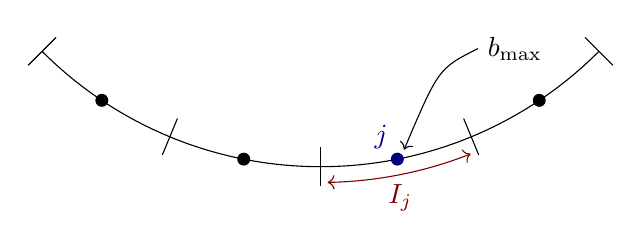
\begin{tikzpicture}
  [scale=5,
  midpoints/.style=blue!50!black,
  intervals/.style=red!50!black]
  \draw (225:1) arc [start angle=225, end angle=315, radius=1];
  \foreach \th in {-2,...,2}
  \draw (270 + 22.5*\th:.95) -- (270 + 22.5*\th:1.05);

  \foreach \th in {236.25,258.75,303.75}
  \filldraw (\th:1) circle [radius=.015];
  
  \filldraw[midpoints] (281.25:1) node [above left] {$\binMidpoint{j}$}
  circle [radius=.015];

  \draw [<->, intervals] (271:1.04) arc [start angle=271, end
  angle=291.5, radius=1.04] node [midway, below] {$I_j$};

  \draw[->] (.4,-.7) node [right,fill=white] {$b_\tn{max}$}
  .. controls (.3, -.75) .. (282.5:.98);
\end{tikzpicture}

%     \caption{Partition of (part of) the platelet surface into
%       $\recAngle$-bins}
%     \label{fig:partition}
%   \end{figure}
% \end{frame}

% \begin{frame}
%   \frametitle{Stochastic algorithm}
%   \begin{itemize}
%   \item Track bonds in a list:
%     \begin{equation*}
%       \mathtt{bondList} = [\wallDist_i, j_i] \quad \tn{where}
%       \quad i = 0, 1, \hdots, \mathtt{numBonds} - 1
%     \end{equation*}
%     \note[item]{The bond list has rows added or removed as bonds form
%       or break. The $\wallDist_i$ values are the
%       $\wallDist$-coordinates of the wall attachment points of each
%       bond, and the $j_i$ values are the bin in which each bond
%       attaches to the platelet.}
%   \item Two parts of a time step in the stochastic simulation:
%     \begin{enumerate}
%     \item Random bond formation and breaking
%     \item Calculating forces and velocities, and updating the position
%       of the platelet
%     \end{enumerate}
%   \item Modified Gillespie algorithm for step 1:
%     \begin{itemize}
%     \item Generate 2 random numbers: one picks the time
%       $\Delta \dTime$ until the next reaction, the other picks which
%       reaction occurs
%     \item Set $\Delta \dTime_\tn{max}$. If $\Delta \dTime > \Delta
%       \dTime_\tn{max}$ then no reactions occur, only the platelet
%       position is updated
%       \note[item]{A maximum time step is enforced because the binding
%         and unbinding rates change as the platelet moves. We don't
%         want these rates to change too much before updating them.}
%       \note[item]{The stochastic method generates the translational
%         and angular velocities, and the number of bonds between the
%         platelet and wall for a single platelet.}
%       \note[item]{Population-wide statistics are generated by running
%         the stochastic algorithm many times}
%       \note[item]{To get a general idea of platelet behavior in the
%         deterministic model, we'll look at results from a simplified
%         system first}
%     \end{itemize}
%   \end{itemize}
% \end{frame}

% \begin{frame}
%   \frametitle{Nondimensionalization}
%   \begin{itemize}
%   \item Both models are nondimensionalized
%   \item Bond density:
%     \begin{multline*}
%       \Pder{\ndBondDensity}{\ndTime} =
%       \ndRotation\Pder{\ndBondDensity}{\recAngle} +
%       \ndVelocity\Pder{\ndBondDensity}{\ndWallDist} +
%       \ndOnConst\exp\left( -\frac{\onForceScale}{2}\ndLength^2\right)
%       \left(1 - \NDReceptorSaturation\right) \\
%       - \exp\left(\offForceScale\ndLength\right)\ndBondDensity 
%     \end{multline*}
%   \item Force and torque balance:
    
%   \end{itemize}
% \end{frame}

% %%%%%%%%%%%%%%%%%%%
% \subsection{Results}
% %%%%%%%%%%%%%%%%%%%
% \begin{frame}
%   \frametitle{Reduced deterministic model: steady state, no saturation}
%   \begin{itemize}
%   \item Both models are nondimensionalized
%     \note[item]{Report results in nondimensional terms}
%   \item Reductions in the deterministic model:
%     \begin{enumerate}
%     \item $\separation = 0$ and $\velocity = \radius\rotation$
%       \note[item]{Platelet is sitting directly on top of the wall, no
%         slip between the two surfaces}
%     \item $\receptorDensity \gg \DimReceptorSaturation$
%       \note[item]{Few bonds form relative to the number of receptors;
%         saturation in the bond formation term is gone}
%     \item Solve for steady states
%     \end{enumerate}
%   \item Nondimensional bond density ($m$):
%     \begin{equation*}
%       0 = \ndRotation\left(\Pder{\ndBondDensity}{\recAngle} +
%         \Pder{\ndBondDensity}{\ndWallDist}\right) +
%       \ndOnConst\exp\left(-\frac{\onForceScale}{2}\ndLength^2\right) -
%       \exp\left(\offForceScale\ndLength\right)\ndBondDensity
%     \end{equation*}
%   \item Torque balance:
%     \begin{equation*}
%       0 = \ndRotFriction\left(\ndAppliedRot - \ndRotation\right) +
%       \ndTotalTorque
%     \end{equation*}
%     \note[item]{This set of equations is solved for a range of omega
%       f's to explore rolling behavior for different parameter values.}
%     \note[item]{Solved backwards}
%     \note[item]{Two dimensional parameters that may change with
%       platelet priming are the basal on rate and the number of
%       receptors on the surface of the platelet}
%     \note[item]{These two dimensional parameters correspond exactly
%       with two nondimensional parameters}
%   \item Important nondimensional parameters: $\ndOnConst =
%     \radius\onConst/\offConst$, $\ndRotFriction = \offConst
%     \rotFriction/(\stiffness\receptorDensity\radius^2)$
%   \end{itemize}
% \end{frame}

% \begin{frame}
%   \frametitle{Reduced deterministic results: Sensitivity to $\onConst$}
%   \begin{figure}
%     \centering
%     \begin{tikzpicture}
  \pgftext{\includegraphics[height=0.7\textheight]{kappa-sweeps-refined}}

  \draw[->] (3.5, 2.8) -- node[rotate=-90, fill=white] {Increasing $\onConst$} +(0, -5);
\end{tikzpicture}
%     \caption{Relation between $\ndRotation$ vs. $\ndTotalTorque$
%       (left) and $\ndAppliedRot$ vs. $\ndRotation$ (right)}
%     \label{fig:kappa-sweeps}
%   \end{figure}
%   \note[item]{These plots show results from a sweep over a range of
%     $\ndRotation$ values, for increasing $\onConst$}
%   \note[item]{The left column shows that the total torque is a
%     non-monotonic function of $\ndRotation$}
%   \note[item]{The torques plotted on the left give the $\ndAppliedRot$
%     required to balance them}
%   \note[item]{The plots on the right are like bifurcation diagrams:
%     show steady states, but no stability info}
%   \note[item]{Dashed line is the angular velocity of an unbound platelet}
%   \note[item]{If we interpret these two branches as stable solution
%     branches, there is bistability, and switches in rolling behavior
%     as $\ndAppliedRot$ changes}
%   \note[item]{With increasing $\ndOnConst$, the bistable region shifts
%     to higher $\ndAppliedRot$s, and the bistable region widens.}
% \end{frame}

% \begin{frame}
%   \frametitle{Reduced deterministic results: Sensitivity to
%     $\receptorDensity$} 
%   \begin{figure}
%     \centering
%     % \includegraphics[height=.8\textheight]{variable-receptors-refined}
%     \begin{tikzpicture}
  \pgftext{\includegraphics[height=0.7\textheight] {variable-receptors-refined}}

  \draw[->] (2.5, 2.8) -- node[rotate=-90, fill=white] {Decreasing $\receptorDensity$} +(0, -5); 
\end{tikzpicture}
%     \caption{Steady state rotation rates for different values of
%       $\receptorDensity$.} 
%     \label{fig:variable-receptors}
%     \note[item]{This is a similar set of plots showing the response of
%       the reduced deterministic model to changes in
%       $\receptorDensity$}
%     \note[item]{Similar to the previous slide, if $\receptorDensity$
%       increases, the bistable region shifts to higher $\ndAppliedRot$
%       and widens}
%     \note[item]{The model responds to priming in the way we expect}
%   \end{figure}
% \end{frame}

% \begin{frame}
%   \frametitle{Model comparison for fixed binding rate (small
%     $\ndOnConst$)}
%   \begin{figure}
%     \centering
%     \input{small-kappa-trials}
%     \caption{Deterministic (red) and stochastic (blue) solutions with
%       $\ndOnConst = 1$. In the left column, means (thick) and means
%       $\pm$ 2 SEM for 1,000 stochastic trials are shown. An example of
%       one stochastic run is shown in the right column.} 
%     \label{fig:small-kappa-trials}
%   \end{figure}
%   \note[item]{The three slides that follow compare results from the
%     deterministic and stochastic models for low, medium, and high
%     values of the basal on rate $\ndOnConst$}
%   \note[item]{The left column compares deterministic (red) with
%     statistics from 1,000 stochastic trials (blue). The thick blue is
%     the mean, and the two thin blue lines are the mean $\pm$ 2 SEM,
%     interpret this like a 95\% confidence interval around the mean.}
%   \note[item]{The right column shows an example stochastic run
%     alongside results from the deterministic model.}
%   \note[item]{From looking at the example stochastic simulation, there
%     are clear jumps and pauses}
%   \note[item]{Also noteworthy, a single bond is capable of bringing a
%     platelet to rest. I think this is why the mean of the stochastic
%     simulation is skewed away from the deterministic simulation.}
% \end{frame}

% \begin{frame}
%   \frametitle{Model comparison for fixed binding rate (intermediate
%     $\ndOnConst$)}
%   \begin{figure}
%     \centering
%     % \includegraphics[width=.75\textwidth]{med-kappa-trials}
%     \begin{tikzpicture}
  \pgftext{\includegraphics[width=0.75\textwidth] {med-kappa-trials}}

  \node at (0, -2.8) {\small Nondimensional time};
  \node[rotate=90] at (-4.3, 1.9) {$\ndVelocity$};
  \node[rotate=90] at (-4.3, 0) {$\ndRotation$};
  \node[rotate=90] at (-4.3, -1.65) {$\mathtt{numBonds}$};
\end{tikzpicture}
%     \caption{Deterministic (red) and stochastic (blue) solutions with
%       $\ndOnConst = 10$. In the left column, means (thick) and means
%       $\pm$ 2 SEM for 1,000 stochastic trials are shown. An example of
%       one stochastic run is shown in the right column.}
%     \label{fig:med-kappa-trials}
%   \end{figure}
%   \note[item]{For the medium $\ndOnConst$, the behavior of the
%     deterministic model has switched to an average velocity of 0}
%   \note[item]{The mean number of bonds in the stochastic model matches
%     up well with the deterministic result, but the velocities are
%     still skewed}
%   \note[item]{The example run mostly remains bound to the surface, but
%     there are jumps in the trajectory}
% \end{frame}

% \begin{frame}
%   \frametitle{Model comparison for fixed binding rate (large
%     $\ndOnConst$)}
%   \begin{figure}
%     \centering
%     % \includegraphics[width=.75\textwidth]{large-kappa-trials}
%     \input{large-kappa-trials}
%     \caption{Deterministic (red) and stochastic (blue) solutions with
%       $\ndOnConst = 50$. In the left column, means (thick) and means
%       $\pm$ 2 SEM for 1,000 stochastic trials are shown. An example of
%       one stochastic run is shown in the right column.}
%     \label{fig:large-kappa-trials}
%   \end{figure}
%   \note[item]{Finally, for large $\ndOnConst$ all of the averages
%     match up well with the deterministic model, and the example run
%     remains bound to the surface, but still translocates due to
%     frequent jumps.}
% \end{frame}

% \begin{frame}
%   \frametitle{Summary of results}
%   \begin{itemize}
%   \item Multiple stable rolling states in deterministic model
%     \vfill
%   \item Model is sensitive to priming (interpreted as changes in
%     $\onConst$ and $\receptorDensity$)
%     \vfill
%   \item Good agreement between the stochastic and deterministic models
%     for large $\ndOnConst$
%     \vfill
%   \item Stochastic model exhibits stepping and pausing
%   \end{itemize}
% \end{frame}

% %%%%%%%%%%%%%%%%%%%
% \section{Short and long-term goals}
% %%%%%%%%%%%%%%%%%%%
% \begin{frame}
%   \frametitle{Overview of short and long-term goals}
%   \note[item]{This is a long list, but the first two items are works
%     in progress, the next two are short term goals, and the last two
%     are long term goals.}
%   \begin{enumerate}
%   \item Use more realistic drag calculations dependent on
%     $\separation$
%     \vfill
%   \item Implement a more efficient stochastic algorithm
%     \vfill
%   \item Compare data from stochastic simulations with experiments:
%     step sizes, pause times, velocity distributions
%     \vfill
%   \item Model multiple types of receptors
%     \vfill
%   \item Implement a 3D model with an ellipsoidal platelet
%     \vfill
%   \item Model intracellular pathways leading to platelet activation
%   \end{enumerate}
% \end{frame}

% \subsection{Work in progress}

% \begin{frame}
%   \frametitle{Work in progress}
%   \note[item]{I'll talk about the work in progress first}
%   \begin{itemize}
%   \item Use more realistic drag calculations (assume that
%     $\separation \ll \radius$)
%     \begin{itemize}
%     \item The force and torque balance equations are coupled
%     \item Finding $\velocity$ and $\rotation$ requires solving a
%       $2\times2$ system
%     \item Drag coefficients depend on $\separation$: Goldman, Cox, \&
%       Brenner (1967)
%     \end{itemize}
%     \vfill
%     \note[item]{For more realistic drag calculation, mention that
%       the current implementation calculates fluid drag assuming that
%       the platelet is far from the wall. There are a set of formulas
%       that approximate the drag on a sphere moving parallel to planar
%       wall. One outcome is that the force and torque balance get
%       coupled in a 2$\times$2 linear system.}
%   \item Implement a more efficient stochastic algorithm
%     \begin{itemize}
%     \item Weakness in the current approach: for biological parameters,
%       the time scale of reactions is slower than the time scale of
%       platelet motion
%     \item Modified Gillespie approach uses a forward Euler time
%       step---stability requires a prohibitively small time step
%     \item A possible solution: using the modified next reaction method
%       (Anderson, 2007)
%     \end{itemize}

%     \note[item]{I will go into a bit more detail on this algorithm,
%       but the first question is why is a more efficient algorithm necessary?}
%   \end{itemize}
% \end{frame}

% \begin{frame}
%   \frametitle{Weaknesses of the modified Gillespie algorithm}
%   \begin{itemize}
%   \item Central problem: for biological parameters the time scale of
%     reactions is slower than the time scale of platelet motion
%     \vfill
%   \item Consequently, with the current algorithm:
%     \begin{enumerate}
%     \item Most random numbers generated by the algorithm are not used
%       \note[item]{When the time to the next reaction is randomly
%         generated, the vast majority of the time it is larger than the
%         maximum allowed time step. This is connected to the second
%         point}
%     \item The time stepping procedure for platelet motion is forward
%       Euler: stability requires a prohibitively small time step
%       \note[item]{It would be nice to use an implicit method, but it
%         isn't clear how to implement that in the framework of modified
%         Gillespie.}
%     \end{enumerate}
%     \vfill
%   \item A possible solution to both problems: the modified next
%     reaction method (Anderson, 2007)
%   \end{itemize}
% \end{frame}

% \begin{frame}
%   \frametitle{Modified next reaction method in platelet rolling}
%   \begin{columns}
%     \begin{column}{.49\textwidth}
%       \begin{itemize}
%       \item Stochastic chemical system with time-varying reaction rates
%       \item Each possible reaction has its own internal time
%       \item Every reaction fires at a unit rate in its internal time
%         \note[item]{Rate the internal clocks advance depends on the
%           rate of the reaction. Clocks associated with reactions with
%           large reaction rates advance quickly. The internal times are
%           basically nondimensional scalings of the absolute time so
%           that each reaction occurs with a unit rate in its internal
%           time}
%       \item Separates the deterministic motion of the platelet from
%         the random bond formation and breaking
%         \note[item]{Addresses both problems from the previous slide:
%           reaction times are never discarded in this method like in
%           the modified Gillespie, and in addition it separates the
%           deterministic motion of the platelet from the random bond
%           formation and breaking.}
%         \note[item]{Use a stiff ODE solver to integrate the platelet's
%           position}
%       \end{itemize}
%     \end{column}
%     \begin{column}{.49\textwidth}
%       \begin{figure}
%         \centering
%         \includegraphics[width=\textwidth]{internal-clocks}
%         \caption{Internal clocks in the modified stochastic method for
%           platelet rolling}
%         \label{fig:internal-clocks}
%       \end{figure}
%     \end{column}
%   \end{columns}
%   \note[item]{This method has not been implemented in the context of
%     rolling models before}
% \end{frame}

% %%%%%%%%%%
% \subsection{Short-term goals}
% %%%%%%%%%%

% \begin{frame}
%   \frametitle{Short-term goals}
%   \begin{itemize}
%   \item Compare data from stochastic simulations with experiments:
%     step sizes, pause times, velocity distributions
%     \note[item]{With the stochastic simulations, it is possible to
%       define step sizes and dwell times in an analogous way to
%       experiments}
%     \vfill
%   \item Model multiple types of receptors
%     \begin{itemize}
%     \item Fast and slow receptors
%     \item Change $N_{T, \tn{slow}}$ and $k_\tn{on, slow}^0$
%       to model priming, change rolling behavior
%     \end{itemize}
%     \note[item]{Include fast and slow receptors in the model, modulate
%       the number of slow receptors (or binding parameters) to model
%       platelet priming}
%   \end{itemize}
% \end{frame}

% %%%%%%%%%%
% \subsection{Long-term goals}
% %%%%%%%%%%

% \begin{frame}
%   \frametitle{Long-term goals}
%   \begin{itemize}
%   \item Implement a 3D model with an ellipsoidal platelet
%     \begin{itemize}
%     \item Use regularized Stokeslets to calculate drag forces and torques
%     \end{itemize}
%     \vfill
%     \note[item]{Modeling a platelet as a sphere is not realistic,
%       because platelets are ellipsoids where the major axes are
%       $\sim$3 times longer than the minor axis. I will expand on this
%       in a couple of slides.}
%   \item Model intracellular pathways leading to platelet activation
%     \begin{itemize}
%     \item Published models---activation by soluble agonists
%     \item Ca$^{++}$ dynamics are important
%     \item Rolling on an immobilized agonist---random stimulation of
%       receptors
%     \end{itemize}
%     \note[item]{The intracellular pathways leading to platelet
%       activation are complex, and it is not obvious how to simplify
%       them. It may not be a feasible goal to integrate a model of
%       intracellular signaling with the rolling model, but the rolling
%       model is informative in how a platelet recieves activation
%       signals from immobilized agonists, and how the rolling behavior
%       responds to activation.}
%   \end{itemize}
% \end{frame}

% \begin{frame}
%   \frametitle{Summary}
%   \begin{itemize}
%   \item Developed a reduced 2D model of platelet rolling with explicit
%     treatment of forces and torques acting on a rolling platelet
%     \vfill
%   \item This model qualitatively reproduces expected rolling behavior
%     \vfill
%   \item Can be extended to incorporate more physical and biological detail
%   \end{itemize}
% \end{frame}
% \begin{frame}
%   \frametitle{Ellipsoidal platelet in 3D}
%   \begin{figure}
%     \centering
%     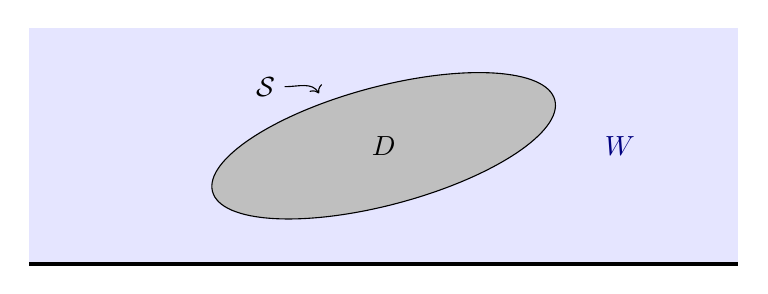
\begin{tikzpicture}[scale=1.5]
  \fill[blue!10] (-3, 0) rectangle (3, 2);
  \draw[very thick] (-3, 0) -- (3, 0);
  \draw[fill=lightgray] (0, 1) circle [x radius=1.5, y radius=.5, rotate=15];
  
  \node[blue!50!black] at (2, 1) {$W$};
  \node at (0, 1) {$D$};
  \node (label) at (-1, 1.5) {$\mathcal{S}$};
  \node (boundary) at (-.5, 1.36) {};
  \draw[->] (label) to [out=0, in=120] (boundary);
\end{tikzpicture}

%     \caption{An ellipsoidal platelet near a plane wall}
%     \label{fig:ellipse}
%   \end{figure}

%   \begin{itemize}
%   \item No analytic expressions for the drag on an ellipsoid
%   \item Need to solve Stokes' equations to find the drag at every time
%     step
%   \item Use regularized Stokeslets to solve Stokes' equations
%   \end{itemize}
% \end{frame}

% \section{}
% \begin{frame}
%   \frametitle{Acknowledgements}
%   \begin{itemize}
%   \item My advisor and my committee
%   \item Anna, Katie, Samantha, \& Hallie
%   \item Biofluids research group
%   \item Proteins-Polymers-Interfaces group
%   \item Funding---NIH Grant 1R01HL126864 'Upstream Priming of
%     Platelets for Adhesion to Biomaterials'
%   \end{itemize}
% \end{frame}

\end{document}
